% \VignetteDepends{corpcor,nlme}
% \VignetteIndexEntry{eigenR2 Tutorial}
% \VignetteKeywords{eigenR2}
% \VignettePackage{eigenR2}
\documentclass[11pt]{article}

\usepackage{epsfig}
\usepackage{latexsym}
\usepackage{amsmath}
\usepackage{amssymb}
\usepackage{amsfonts}
\usepackage{amsxtra}
\usepackage{graphicx,subfigure}
\usepackage{vmargin}

\newcommand{\Robject}[1]{{\texttt{#1}}}
\newcommand{\Rfunction}[1]{{\texttt{#1}}}
\newcommand{\Rpackage}[1]{{\texttt{#1}}}
\newcommand{\Rclass}[1]{{\texttt{#1}}}
\newcommand{\Rmethod}[1]{{\texttt{#1}}}
\newcommand{\Rfunarg}[1]{{\texttt{#1}}}

\parindent 0in
\setpapersize{USletter}
\setmarginsrb{1truein}{0.5truein}{1truein}{0.5truein}{16pt}{30pt}{0pt}{20truept}
\setlength{\emergencystretch}{2em}
\usepackage{/Library/Frameworks/R.framework/Versions/2.6/Resources/share/texmf/Sweave}
\begin{document}

\title{Bioconductor's eigenR2 package}
\author{Lin S. Chen and John D. Storey \\
Lewis-Sigler Institute \\
Department of Molecular Biology \\
Princeton University \\
email: \texttt{lschen@princeton.edu}}

\maketitle
\bibliographystyle{plain}
\tableofcontents


\section{Overview}

Eigen-$R^2$ is a high-dimensional version of the classic $R^2$ statistic.  It can be applied to determine the aggregate $R^2$ value for many related response variables according to a common set of independent variables. The \Rpackage{eigenR2} package contains functions for estimating eigen-$R^2$; see \cite{chen2008} for more details about the algorithm.\\

This document provides a tutorial for using the \texttt{eigenR2} package.  The package contains a function \Rfunction{eigenR2} that estimates eigen-$R^2$ for variables of interest and a plot function \Rfunction{plot.eigenR2} to graphically display information about the right eigenvectors used in calculating eigen-$R^2$. Detailed information on functions can be obtained in the help files. For instance, to view the help file for the function \Rfunction{eigenR2} within R, type \texttt{?"eigenR2"}.  Here we illustrate the use of \Rfunction{eigenR2} with some simulated examples. We show how to estimate conditional eigen-$R^2$ values, and how to adjust the estimate of eigen-$R^2$ for small samples. We provide the option to obtain further ``denoised'' versions of eigen-$R^2$ by specifying a significance threshold for the right eigenvectors. The function \Rfunction{sva.id} \cite{leek2007} tests the null hypothesis for each eigenvector that it explains more variation than would be expected by chance. The function selects only the significant eigenvectors to estimate eigen-$R^2$, according to a user-chosen p-value threshold.  We also show how to user can specificy more elaborate model to estimate eigen-$R^2$, e.g., using linear mixed effect model. 

  
\section{Simulated Data}

We simulated a gene expression array data set along with several independent variables to illustrate the estimation of eigen-$R^2$. The simulated data used in this analysis is also included in the \Rpackage{eigenR2} package as the dataset \texttt{eigSdat}. This data set consists of two parts. The first part \texttt{varList} contains three variables acting as the independent variables: \texttt{age}, \texttt{genotype} and \texttt{ID}. The second part \texttt{exp} is a 200 genes by 50 arrays gene expression matrix, in which all the genes are associated with age and genotype according to varying effect sizes. Each row of the expression matrix can be thought of as a response variable in a regression.  

One can load the data set by typing \texttt{data(eigSdat)}.

\begin{Schunk}
\begin{Sinput}
> library(eigenR2)
> data(eigSdat)
> names(eigSdat)
\end{Sinput}
\begin{Soutput}
[1] "varList" "exp"
\end{Soutput}
\begin{Sinput}
> dim(eigSdat$varList)
\end{Sinput}
\begin{Soutput}
[1] 50  3
\end{Soutput}
\begin{Sinput}
> dim(eigSdat$exp)
\end{Sinput}
\begin{Soutput}
[1] 200  50
\end{Soutput}
\end{Schunk}


\section{The \Rfunction{eigenR2} function}

The \Rfunction{eigenR2} function estimates eigen-$R^2$ for one variable or a set of variables of interest in high-dimensional data.\\

In the following example, \Rfunction{eigenR2} function estimates the eigen-$R^2$ for \texttt{age} in the expression data. By default, we center each row according to the null model, which is simply the average value for each respective response variable. Note that if each response variable is scaled to have mean zero and variance one, then eigen-$R^2$ is equal to mean-$R^2$.  In this example, right eigenvectores are called ``eigen-genes.''


\begin{Schunk}
\begin{Sinput}
> mod1 <- model.matrix(~1+age)
> eigenR2.age <- eigenR2(dat = exp, model = mod1)
> eigenR2.age$eigenR2
\end{Sinput}
\begin{Soutput}
[1] 0.0904609
\end{Soutput}
\end{Schunk}


One can also adjust the eigen-$R^2$ estimates according to sample size. Set the option \texttt{adjust =  TRUE}, and sample size adjustment will be performed. 
\begin{Schunk}
\begin{Sinput}
> eigenR2.age.adj <- eigenR2(dat=exp, model=mod1, adjust=TRUE)
> eigenR2.age.adj$eigenR2
\end{Sinput}
\begin{Soutput}
[1] 0.07151217
\end{Soutput}
\end{Schunk}

By specifying a significance threshold for eigen-genes in the optional argument \texttt{eigen.sig}, one can select to use only the statistically significant eigen-genes in computing the eigen-$R^2$ \cite{leek2007}. If no eigen-genes are significant at the user-chosen p-value threshold, it indicates the data contain all noise and no structure, and no independent variables contribute significantly to the variation in the response variables. In that case, the function will return zero as the eigen-$R^2$ estimate.

\begin{Sinput}
> eigenR2.age.adj2 <- eigenR2(dat=exp, model=mod1, eigen.sig=0.01)
> eigenR2.age.adj2$eigenR2
\end{Sinput}
\begin{Soutput}
[1] 0.08910577
\end{Soutput}


The function can also compute the conditional eigen-$R^2$ by specifying a null model \texttt{null.model}. For example, it computes the eigen-$R^2$ of genotype given age by 
\begin{Schunk}
\begin{Sinput}
> mod2 <- model.matrix(~1+age+as.factor(geno))
> eigenR2.g <- eigenR2(dat=exp, model=mod2, null.model=mod1)
> eigenR2.g$eigenR2
\end{Sinput}
\begin{Soutput}
0.09296529
\end{Soutput}
\end{Schunk}

By default, a linear model fit by least squares will be used to estimate $R^2$ values. Note that basis methods can also be employed as a linear operator applied to minimize the residual sum of squares. If the estimation function \texttt{mod.fit.func} is provided, one can estimate $R^2$ using other model fitting techniques, e.g., linear mixed effect models. Note, \texttt{mod.fit.func} has to be a function to estimate $R^2$ but not conditional $R^2$ values. Estimating conditional $R^2$ with flexible function is currently not provided in this package. 

Here we provide an example showing how to estimate eigen-$R^2$ using a linear mixed effect models \Rfunction{lme}. 

\begin{Schunk}
\begin{Sinput}
> library(nlme)
> func2 <- function(y) {
+       m1 <-lme(y~1+age+as.factor(geno), random=~1|ID)
+       r2 <- 1-sum(resid(m1)^2)/sum((y-mean(y))^2)
+       return(r2)
+   }
> eigenR2.ag <- eigenR2(dat=exp, mod.fit.func=func2)
> eigenR2.ag$eigenR2
\end{Sinput}
\begin{Soutput}
[1] 0.2239942
\end{Soutput}
\end{Schunk}



\section{The \Rfunction{plot.eigenR2} function}

The \Rfunction{plot.eigenR2} graphically displays information on the right eigenvectors. It displays:  
\begin{enumerate}
    \item A plot that shows the proportion of total variation each eigenvector captures.
    \item A plot of the $R^2$ for the significant eigenvectors. Note that if the optional significance threshold \texttt{eigen.sig} is not provided, all the eigenvectors are treated as significant.
    \item A plot of the p-values for each eigenvector, if ``eigen.sig'' is specified.
\end{enumerate}

For example, 
\begin{Schunk}
\begin{Sinput}
> plot.eigenR2(eigenR2.age.adj2)
> plot.eigenR2(eigenR2.ag)
\end{Sinput}
\end{Schunk}

\bibliography{eigenR2} 

\newpage
\begin{figure}[ht]
  \begin{center}
    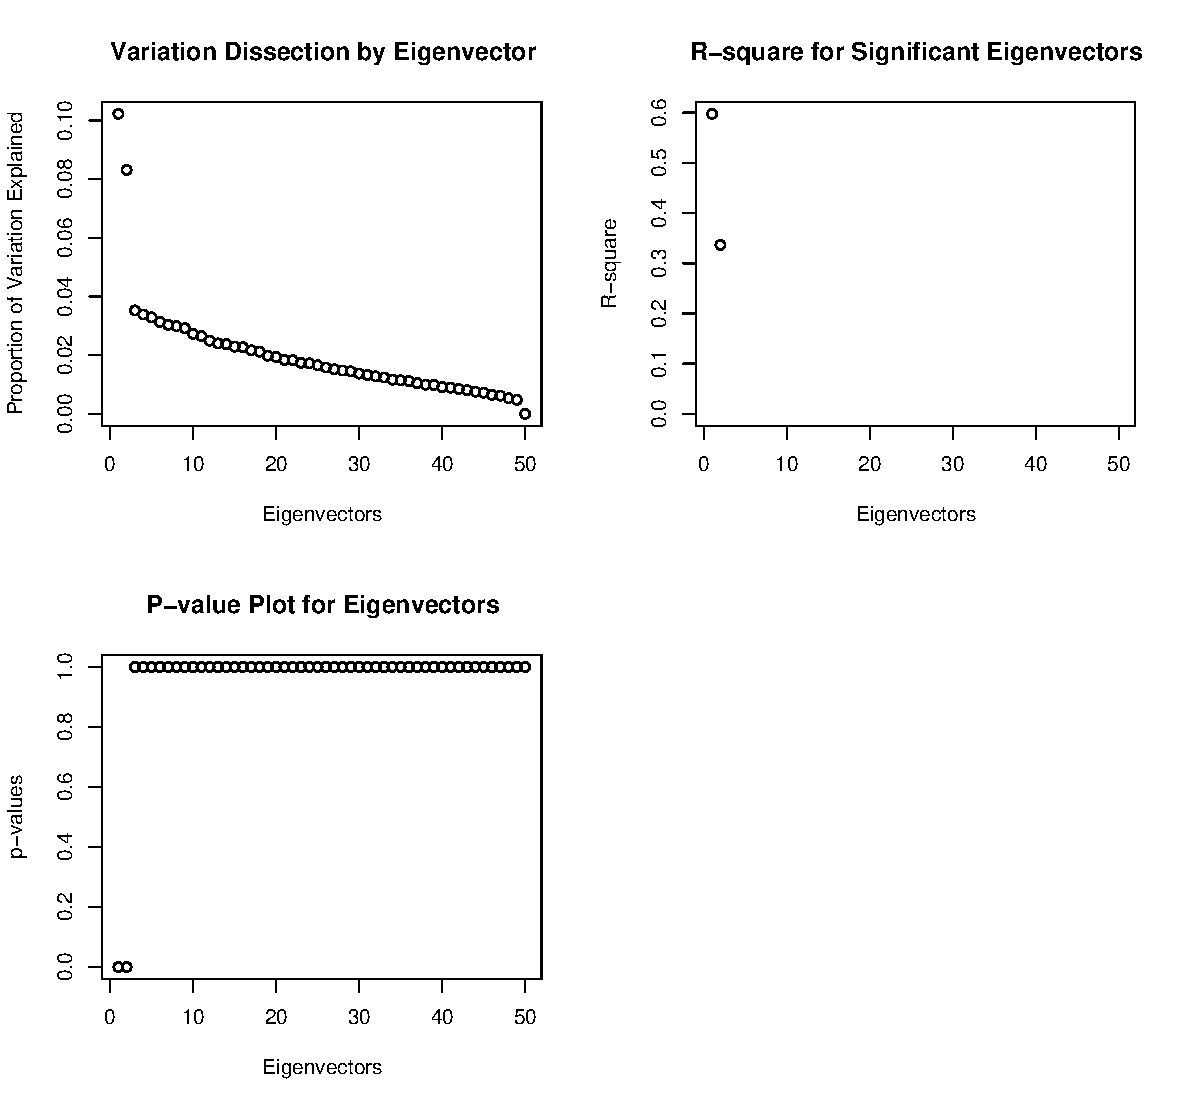
\includegraphics[width=6in,height=6in]{ageadj2}
  \end{center}
  \caption{An example of an eigenR2 plot.}
\end{figure}
\begin{figure}[ht]
  \begin{center}
    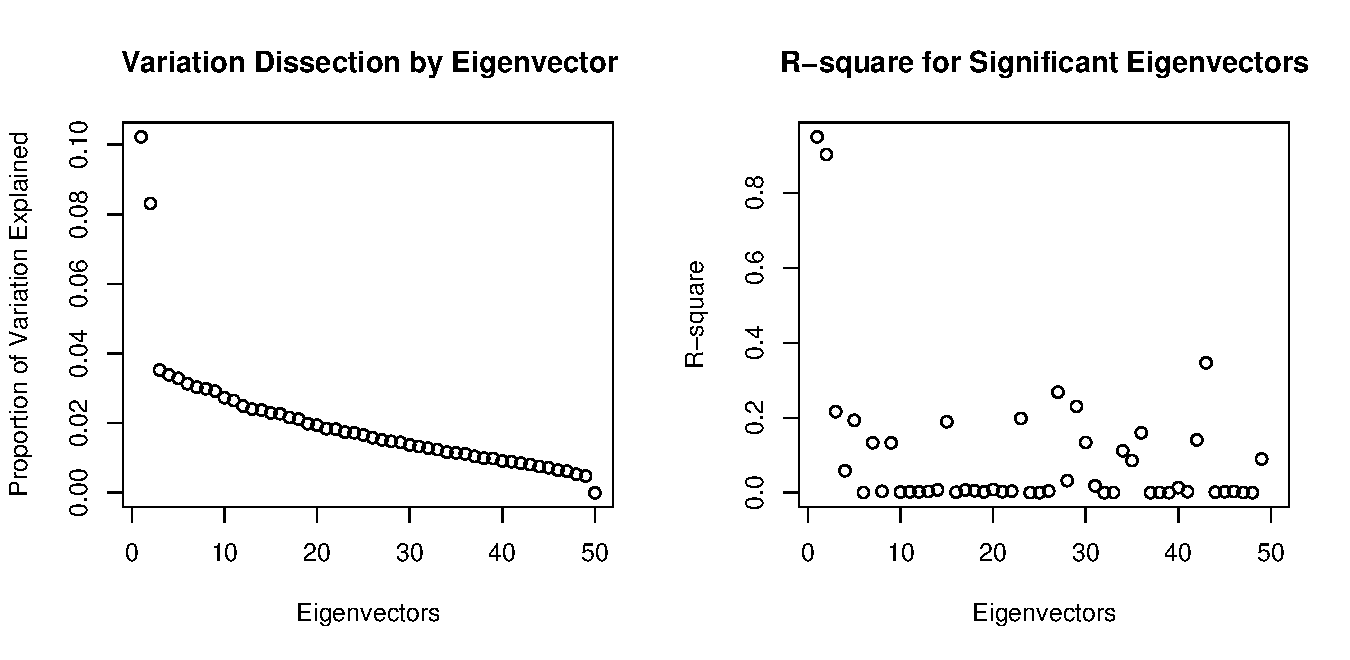
\includegraphics[width=6in,height=3in]{ag}
  \end{center}
  \caption{A second example of an eigenR2 plot.}
\end{figure}


\end{document}
